\documentclass[15pt,a4paper]{article}
\usepackage{tikz}
\usepackage{graphicx}
\usepackage{amsmath}
\graphicspath{ {images/} }
\usepackage{multirow}
\usepackage{caption}
\usepackage{subcaption}
\usepackage[left=1.5in, right=1.5in, top=1.5in, bottom=1.5in]{geometry}
\usepackage{titling}
\usetikzlibrary{shapes,decorations,arrows}
\tikzstyle{cloud} = [draw, ellipse]
\tikzstyle{block} = [rectangle, draw,text centered]
\tikzstyle{line} = [draw, -latex']
\tikzstyle{decision} = [diamond, draw]

% centering the title vertically
\renewcommand\maketitlehooka{\null\mbox{}\vfill}
\renewcommand\maketitlehookd{\vfill\null}

\begin{document}
\title{\textbf{Software Systems Lab 7:\\
TeX Lab\\}}
\author{Team CodeWarriors}
\date{02 September 2018}
\begin{titlepage}
\maketitle
\pagenumbering{gobble}
\end{titlepage}

\newpage

\pagenumbering{arabic}
\begin{figure}
\centering
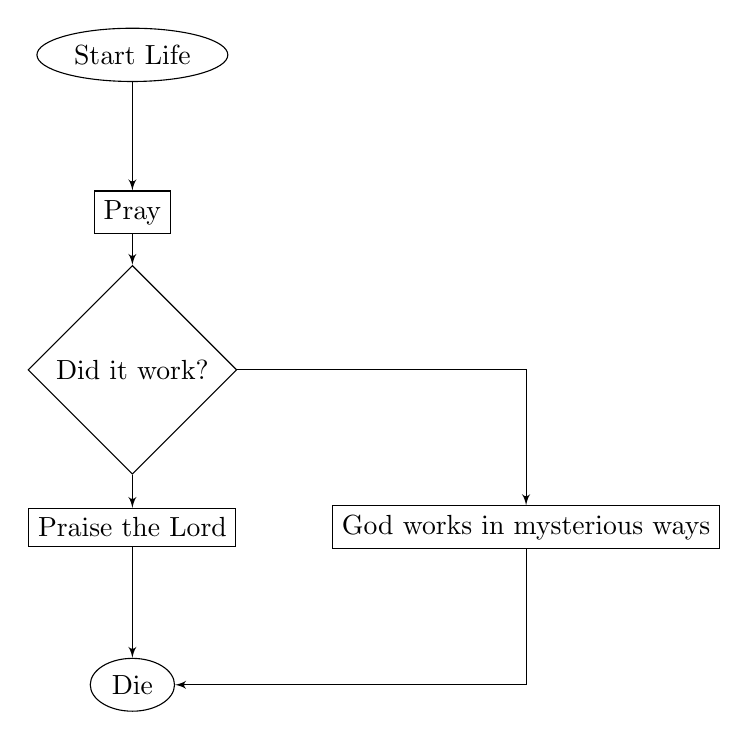
\begin{tikzpicture}[node distance=2cm]

\centering

\node[cloud](start){Start Life};
\node[block,below of=start](pray){Pray};
\path [line] (start) -- (pray);
\node[decision,below of=pray](did){Did it work?};
\path [line] (pray) -- (did);
\node[block,below of=did](praise){Praise the Lord};
\path [line] (did) -- (praise);
\node[block,right of=praise,node distance=5cm](god){God works in mysterious ways};
\path [line] (did) -| (god);
\node[cloud,below of=praise](die){Die};
\path[line] (praise) -- (die);
\path[line] (god)|-(die); 


\end{tikzpicture}
\caption{Flowchart of a theist life}
\end{figure}



\par
\vspace{5mm}
Figure 1 above refers to a funny conundrum theists are believed to be
living in by the atheists. This is just a joke I picked up from some forum,
not taking sides, not even a bit. This is how scared social media has made
us, We can not pick sides. Moving on . . . . You need to know how to cite
papers in \LaTeX. For e.g. you are talking about research on Indowordnet
[1], in that case such a citation must be used near a name.  In case you
need to quote the authors of a paper in a statement, instead of citing them
against a topic or word or a line, you need to use a different kind of citation
methodology.

\newpage

\begin{table}[]
\caption{Table depicting the use of both multirow and multicolumn}
\centering
\begin{tabular}{ |c|c|c|c|c|c|c|c|c|c|c| }
\cline{3-11}
\multicolumn{2}{c|}{}&
\multicolumn{5}{|c|}{\textbf{Basic Properties}} & \multicolumn{4}{|c|}{\textbf{Readability}}\\
\cline{3-11}
\multicolumn{2}{c|}{}&
\textbf{WC} & \textbf{SC} & \textbf{C-W} & \textbf{S-W} & \textbf{W-S} & \textbf{FK} & \textbf{GF} & \textbf{SMOG} & \textbf{LEX}\\
\hline
\multirow{2}{*}{\textit{Baseline}} & Mean & 0.84
& 0.41
& \textbf{0.56}
& \textbf{0.46}
& \textbf{0.55}
& \textbf{0.60}
& 0.56
& 0.57
& 0.63\\

\cline{2-11}
& SD
& 0.07
& 0.08
& 0.06
& 0.07
& 0.05
& 0.05
& 0.06
& 0.07
& 0.05\\
\hline
\hline
\multirow{2}{*}{\textit{ScaComp\textsubscript{h}}} & Mean & 0.84
& 0.41
& \textbf{0.56}
& \textbf{0.46}
& \textbf{0.55}
& \textbf{0.60}
& 0.56
& 0.57
& 0.63\\

\cline{2-11}
& SD
& 0.07
& 0.08
& 0.06
& 0.07
& 0.05
& 0.05
& 0.06
& 0.07
& 0.05\\
\hline
\hline
\multirow{2}{*}{\textit{ScaComp\textsubscript{l}}} & Mean & 0.84
& 0.41
& \textbf{0.56}
& \textbf{0.46}
& \textbf{0.55}
& \textbf{0.60}
& 0.56
& 0.57
& 0.63\\

\cline{2-11}
& SD
& 0.07
& 0.08
& 0.06
& 0.07
& 0.05
& 0.05
& 0.06
& 0.07
& 0.05\\
\hline



\end{tabular}


  
\end{table}
\par

To combine rows a package must be imported with in your preamble, then
you can use the XXXXXXX command in your document, I did it.  The
table below includes mathematical notations, which you can produce by
embedding the expression in \textdollar \ \ \textdollar \ 
delimiters. For subscript, use underscore
and for superscript, use carrot.
\par
\vspace{5mm}

{\Large In table 1 above, we try to demonstrate all the features
required to be demonstrated in a table.  We use multiple
newline, we use a package to enable the use of multiple rows,
and multiple columns in the table.  Additionally, We have
also drawn lines from specific column to column. We also
use box resizing with a width specifier for resizing the box
within the limits of the document, and avoid any overflow. }

\par
\vspace{5mm}

Now, we will import images side by side in the same document
\newpage



\begin{figure}
\centering
\begin{minipage}{.5\textwidth}
  \centering
  \includegraphics[width=5cm]{fig1.png}
  \captionof{figure}{First figure}
  \label{fig:test1}
\end{minipage}%
\begin{minipage}{.5\textwidth}
  \centering
  \includegraphics[width=5cm]{fig2.png}
  \captionof{figure}{Second figure}
  \label{fig:test2}
\end{minipage}
\end{figure}

\par
The images have been put in, and they are side by side in the same docu-
ment on the same page. We have used the package floatrow and graphicx to
import images on Page 3. The images are some random screenshots of my
phone. I am adding an mathematical equation now just for the sake of it,
because I think this is the only thing left to be demonstrated.

\begin{equation} \label{nll}
NLL=\sum_{i=1}^{N}\log(P(s_i))
\end{equation}

\begin{flushleft}
where
\textit{s\textsubscript{i}} 
is the length of the \textit{i}\textsuperscript{th} saccade.
\end{flushleft}

\newpage

\begin{figure}
    \centering
    \begin{subfigure}[b]{0.4\textwidth}
        \centering
        \includegraphics[width=\textwidth]{fig3_a.jpg}
        \caption{Caption 1}
    \end{subfigure}
    \hfill
    \begin{subfigure}[b]{0.4\textwidth}
        \centering
        \includegraphics[width=\textwidth]{fig3_b.jpg}
        \caption{Caption 2}
    \end{subfigure}
    \caption{Caption for this figure with two images}
\end{figure}


This is another alternative to posting images in a \LaTeX \ Document, although you would still want me to put them in a table, since ‘The Document’
had them in a table. Let me try to do that.

\vspace{10mm}
\begin{figure}[htb]
    \includegraphics[width=0.45\textwidth]{fig4.png}%
    \hspace*{\fill}% induce some horizontal separation between images 1 and 2
    \includegraphics[width=0.45\textwidth]{fig5.png}

    \includegraphics[width=0.45\textwidth]{fig5.png}%
    \hspace*{\fill}% induce some horizontal separation between images 3 and 4
    \includegraphics[width=0.45\textwidth]{fig4.png}
\end{figure}

Now, that we have all the possible ways multiple images can be aligned in
the table. We will conclude this document with the final section.

\newpage

\section*{Conclusion}
This document comprehensively demonstrated the capabilities of \LaTeX \ as a
document typesetting / desktop publishing package. We have used various
font size / family settings, we have used verbatim to display Latex code
in a latex document, image settings, sections, subsections, references using
labels, mathematical equations, notations, use of  for creating
a diagram / flowchart etc.  I hope this suffices the need of learning basic \LaTeX. I hope you also notice that the last section i.e. Conclusion on Page
5 is unnumbered and displays the use of something.


\begin{thebibliography}{9}
\bibitem{latexcompanion} 
Pushpak Bhattacharyya. Indowordnet. In 
\textit{The WordNet in Indian Languages}, 
pages $1\hat{a}\Breve{A}{{\c{S}}}18$.  Springer, 2017.
\end{thebibliography}
\end{document}
